\documentclass[12pt]{article}

\title{Math Foundations}
\author{Abel Doñate}
\date{}

\usepackage{amsmath}
\usepackage{hyperref}
\usepackage{graphicx}
\graphicspath{ {./images/} }
\usepackage{wrapfig}

\setcounter{page}{0}

%Geometry
\usepackage{geometry}
\geometry{a4paper, margin=1in}


\begin{document}

\maketitle
\tableofcontents
\newpage

\section{Useful techniques to solve problems}
    \subsection{The Well ordered principle and Descent to infinity}
    The well ordering principle tells us that we cannot have a sequence of non-negative integers such that $a_1>a_2>...$.
    This is useful to apply in descent to infinite proofs. \\ \\
    Suppose you have a problem in which you are given a condition and you have to check what numbers satisfy the condition. In this case you can apply descent to infinite:
    \begin{itemize}
        \item[1)] Find a condition that guarantees you that a set of numbers satisfy the condition if and only if another set of numbers that are strictly less then the original set satisfy the condition.
        \item[2)] By the Well ordering principle, reason that it is impossible to keep descending infinitely many times , so the sequence must stop somewhere.
        \item[3)] If we can apply it many times, that means that there is no set of numbers that satisfy the condition (or only does the trivial ones like $(0,0,0)$).
    \end{itemize}
    A good example is to find the triples $(a, b, c)$ that satisfy $a^3 + 2b^3 = 4c^3$.\\
    Because the right hand side (RHS) is even, then $a$ must be even $\implies a=2x$. \\
    Dividing by $2$ the equation is $4x^3 + b^3 = 2c^3$ \\
    Because RHS is even, then $b$ must be even $\implies b=2y$. \\
    Dividing by $2$ the equation is $2x^3 + 4y^3 = c^3$ \\
    Because LHS is even, then $c$ must be even $\implies c=2z$. \\
    Dividing by $2$ the equation is $x^3 + 2y^3 = 4z^3$ \\
    
    We observe that we are left with the original case. That tells us that $(a, b, c)$ only holds if $(a/2, b/2, c/2)$ also holds. Applying descent to infinity, we assure that there is no solution except the trivial one $(0,0,0)$
    
    \subsection{Mathematical induction}
    We can prove lots of types of problem by this simple principle. \\
    
    Suppose we have to prove that a given condition holds for every natural number. Then one way to prove it is to check if holds for $k=1$, and then prove that if it holds for $k$, then, it must hold for $k+1$. \\
    
    The sketch of the steps is the following:
    \begin{itemize}
        \item[1)] \textbf{Base case.} First we prove that the condition holds for $k=1$ (or the first element of the set you are given).
        \item[2)] \textbf{Induction statement.} Now we prove that if $k$ holds, then $k+1$ also holds.
        \item[3)] \textbf{Proof.} Finally you reason that the problem has been solved by the principle of mathematical induction 
    \end{itemize}
    
    \subsection{Double counting}
    Sometimes it is useful to exploit different perspectives of a problem. If your task is to prove an equivalence, perhaps the easiest way to do it is double counting, or compute the expression in two different ways, but showing that both are equal.
    
\section{Inequalities}
    \subsection{Means inequalities}
    We have the chain of inequalities $HM\leq GM\leq AM\leq QM$:
    \[\frac{1}{\frac{1}{a}+\frac{1}{b}+\frac{1}{c}}\leq \sqrt[3]{abc}\leq \frac{a+b+c}{3}\leq \sqrt{\frac{a^2+b^2+c^2}{3}} \]
    The equality holds when $a=b=c$.
    
    \subsection{Cauchy's inequality}
    \[\vec{a}\cdot \vec{b}\leq |\vec{a}||\vec{b}| \implies \left(\sum{a_ib_i}\right)^2 \leq \left(\sum{a_i^2}\right)\left(\sum{b_i^2}\right) \]
    
    \subsection{Chebyshev's inequality}
    If we have two ordered vectors (both increasing or decreasing):
    \[n\sum{a_ib_i}\geq \left(\sum{a_i}\right)\left(\sum{b_i}\right)\geq n\left(\sum{a_ib_{n+1-i}}\right)\]
    
    \subsection{Jensen's inequality}
    Let $f$ be a convex function (i.e. $f''\geq 0$). Then:
    \[f\left(\sum{\alpha_ix_i}\right) \leq \sum{\alpha_i f(x_i)} \ \ \ \ \ where \ \ \sum{\alpha_i}=1\]


\section{Combinatorial numbers}
    The number of ways to choose k elements in a set of n elements is \textit{n choose k}:
    \[\binom{x}{k}=\frac{n!}{k!(n-k)!}\]
    Some of the properties of combinatorial numbers are:
    \begin{align} 
        (x+y)^n &= \sum{\binom{n}{k}x^ny^{n-k}} \\
        \binom{n+m}{k} &= \sum{\binom{n}{i}\binom{m}{k-i}} \ \ \ \text{(Vandermonde's identity)}
    \end{align}
    
    \begin{wrapfigure}{r}{0.23\textwidth}
        \centering
        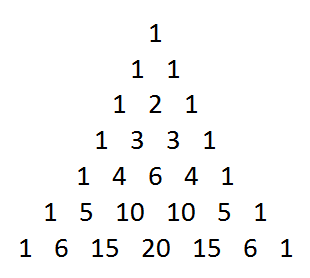
\includegraphics[width=0.23\textwidth]{pascal}
    \end{wrapfigure}
    
    These numbers appear also in Pascal's triangle. The ith element of the nth row (begining both with 0) is $\binom{n}{i}$.\\ \\
    An extension of \textit{n choose k} is the following:
    \[\binom{n}{k_1 \cdots k_m}=\frac{n!}{k_1!\cdots k_m!}\]
    and it appears in the multinomial theorem:
    \[(x_1+\cdots +x_m)^n=\sum_{k_1+ \cdots +k_m=n}{\binom{n}{k_1 \cdots k_m}x_1^{k_1}\cdots x_m^{k_m}}\]


\section{Sets}
    \subsection{Operations and De Morgan's Law}
    Main operations
    \begin{itemize}
    	\item Union. $A \cup B$
    	\item Intersection $A \cap B$
    	\item Difference $A \setminus B$ or $A-B$
    	\item Symmetric difference $A \bigtriangleup B = (A\cup B)-(A\cap B)$
    	\item Complement. $\bar{A}$	
    \end{itemize}
    \textbf{De Morgan's Law:}
    \begin{itemize}
    	\item $\overline{A \cup B}=\bar{A}\cap \bar{B}$
    	\item $\overline{A\cap B}=\bar{A}\cup \bar{B}$
    \end{itemize}

	\subsection{Canonical decomposition}
	Every function $f$ can be decomposed in a surjective, bijective and injective functions. 		For instance: $f=i \circ b \circ \pi$.
	\begin{itemize}
		\item $\pi$ maps to its equivalence class
		\item $b$ maps to the function of every equivalence class
		\item $i$ maps to itself
    \end{itemize}
    \section{Algebraic structures}
	\subsection{Group}
	A group is a set with one binary operation $(S,\star)$ that must satisfy:
	\begin{itemize}
		\item Closure under $\star$
		\item Associative $(a\star b)\star c=a\star (b\star c)$
		\item Identity element $e$ such that $e\star a=a\star e=a$
		\item Inverse element. Every $a$ has an inverse $a^{-1}$
	\end{itemize}
	
	If the group is commutative $a\star b= b\star a$, then is called \textbf{Abelian}. \\
	
	Examples of abelian group are $\mathbf{Z}_n$ (group whose elements are $0, 1, \cdots, n-1$, and the operation is the sum modulo n), or the group or rotations of a regular polygon. \\
	
	An example of non-abelian group is the group of rotations of a cube. The proof is left to the reader.
	
	\subsection{Ring}
	A Ring is a set with two binary operations $(S,\star, \top)$ that must satisfy:
	\begin{itemize}
		\item $(S, \star)$ is an abelian group
		\item Distributive $a\top (b\star c)= (a\top b) \star (a\top c)$
		\item Identity elements $e_\star, e_\top$
	\end{itemize}
	
	If $e_\star \neq e_\top$ and $a\top b\neq e_\star$, then is called an \textbf{Integral domain}.\\
	
	One example of a Ring is $\mathbf{Z}$ with usual sum and product.\\
	
	$\mathbf{Z}_p$ with $p$ prime is an example of an integral domain. $\mathbf{Z}_6$, because 6 is not prime, is not an integral domain, as $2\times 3=0=e_+$. 
	
	\subsection{Field}
	A field is a ring with no inverse for $e_\star$ under $\top$.\\
	
	The most common example is $\mathbf{R}$. Observe that the element $0=e_+$ has no inverse under multiplication.
	
\section{Stereographic projection}
    \begin{wrapfigure}{r}{0.30\textwidth}
        \centering
        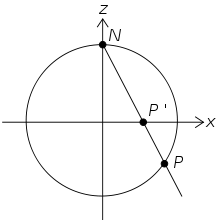
\includegraphics[width=0.30\textwidth]{stereo1}
    \end{wrapfigure}
    
    The stereographic projection maps every point in a sphere except the upper pole to the $XY$ plane. On the other hand we can take the inverse stereographic projection, that maps every point in the plane to the sphere (except the upper pole). \\
    
    This map is achieved by drawing a line from the upper pole to the point in the sphere and taking the intersection with the $XY$ plane. \\
    
    If we define the coordinates of the plane as $x, y$ as usual and the coordinates of the sphere as $\alpha, \beta, \gamma$, we can derive the following equations:
    \[F(\alpha, \beta, \gamma)=\left(\frac{\alpha}{1-\gamma}, \frac{\beta}{1-\gamma}\right) \ \ \ \
    F^{-1}(x, y)=\left(\frac{2x}{x^2+y^2+1}, \frac{2y}{x^2+y^2+1}, \frac{x^2+y^2-1}{x^2+y^2+1}\right)\]

\end{document}
